\capitulo{SISTEMA DESENVOLVIDO}

Será desenvolvido um sistema que otimiza a alocação das salas facilizando a vida do gerente. Por se tratar de um problema especifico fica dificil encontrar tecnlogias disponiveis para a resolução do problema sendo assim necessario o atendimento de um sistema que atenda todas as necessisdades exigidas.

\secao{Modelagem}

Arrumar referencia.\par

Segundo Booch et al. (2001) a modelagem de um diagrama de caso de uso é uma
técnica usada para descrever e definir os requisitos funcionais de um sistema. Para sistemas
que possuem um número elevado de funcionalidades, a construção destes diagramas visa
facilitar o entendimento do problema, a documentação do que será desenvolvido bem
como facilita o próprio desenvolvimento.


\subsecao{Diagramas de entidade relacionamento}

Arrumar referencia.\par
Por se tratar de uma aplicação de banco de dados, a modelagem de dados foi
também construída. Segundo Elmasri & Navathe (2005) a modelagem conceitual é uma
fase muito importante no planejamento de uma aplicação de um banco de dados bem
sucedida.
Ainda segundo Elmasri & Navathe (2005), o modelo relacional representa o banco
de dados como uma coleção de relações. Informalmente, cada relação se parece com uma
tabela de valores.
Na Figura 3.8 tem-se o diagrama para o esquema do banco de dados relacional do
sistema. Cada tabela é chamada de relação e cada cabeçalho de coluna é conhecido como
atributo. Os atributos sublinhados em cada tabela indicam a chave-primária e a indicação
“(FK)” exibe a chave-estrangeira em cada relação.

\begin{figure}[!htb]
\caption[Diagrama de componetes do sistema xxx]{Diagrama de componetes do sistema xxx}
\label{fig:figura1}
\centering
\includegraphics{images/diagramaComponentes.png}
\\ \textbf{\footnotesize Fonte: Desenvolvido pelo autor}
\end{figure}


\subsecao{Diagramas de caso de uso}


A Figura 3.4 descreve todas as funcionalidades que o usuário de perfil
“Administrador” poderá executar na ferramenta.


\begin{figure}[!htb]
\caption[Diagrama de componetes do sistema xxx]{Diagrama de componetes do sistema xxx}
\label{fig:figura1}
\centering
\includegraphics[scale=0.8]{images/diagramaComponentes.png}
\\ \textbf{\footnotesize Fonte: Desenvolvido pelo autor}
\end{figure}

Já a Figura 3.5 apresenta as funcionalidades que o usuário de perfil Consulta pode
executar. A seta partindo do usuário Administrador indica que este pode executar qualquer
funcionalidade que o usuário Consulta tem acesso.

\begin{figure}[!htb]
\caption[Diagrama de componetes do sistema xxx]{Diagrama de componetes do sistema xxx}
\label{fig:figura1}
\centering
\includegraphics{images/diagramaComponentes.png}
\\ \textbf{\footnotesize Fonte: Desenvolvido pelo autor}
\end{figure}



\subsecao{Diagramas de classe}

Segundo Booch et al. (2001), Diagrama de Classes demonstram a estrutura estática
das classes de um sistema, onde estas representam as “coisas” que são gerenciadas pela
aplicação modelada. Ainda segundo Booch et al. (2001), uma classe num diagrama pode
ser diretamente implementada utilizando-se uma linguagem de programação orientada a
objetos, no caso deste trabalho, a Linguagem Java.
A partir da Figura 3.7 pode-se observar as classes manipuladores do sistema. Elas
estão identificadas, descritas com seus métodos e relacionadas entre si. Geralmente um
sistema possui mais de um diagrama, pois nem todas se encaixam em um diagrama
específico.

\begin{figure}[!htb]
\caption[Diagrama de componetes do sistema xxx]{Diagrama de componetes do sistema xxx}
\label{fig:figura1}
\centering
\includegraphics{images/diagramaComponentes.png}
\\ \textbf{\footnotesize Fonte: Desenvolvido pelo autor}
\end{figure}
%==============================================%

\secao{Algoritimo Genético}


O primeiro passo a ser dado para o desenvolvimento do algoritimo é o pleno conhecimento do problema e a ligação entre os termos utilizados na biologia com os itens do problema proposto anteriormente. Foram utilizadas varias fontes para o desenvolvimento do trabalho, porem foram feitas modificação para que o modelo tratado por outros autores funcionasse como necessario.\par

Para o melhor entendimento dos passos tomados durante a interpretação do problema e da sua ligação com o algoritmo genetico será criado um pequeno ambiente de alocação. Este ambiente contem as seguintes propriedades, três salas, seis horarios, sete dias da semana, cinco discplinas, e 9 relacionamentos de obrigatoriedade entre discplina e horário.\par

\begin{figure}[!htb]
\caption[Representação do ambiente]{Representação do ambiente}
\label{fig:figura1}
\centering
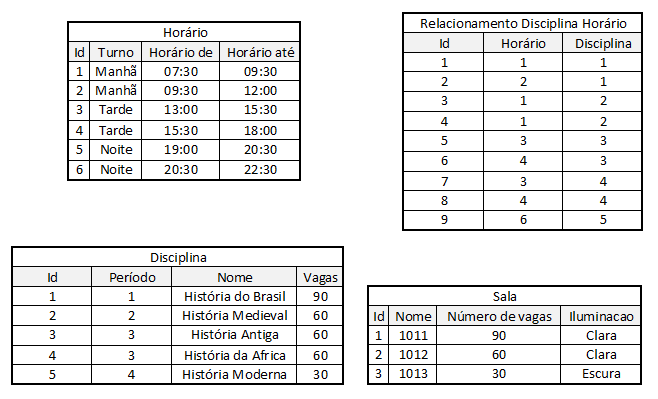
\includegraphics{imagens/representacaoAmbiente.png}
\\ \textbf{\footnotesize Fonte: Desenvolvido pelo autor}
\end{figure}

\subsecao{Individuo}

	Alguns trabalhos tratam cromossomos e inidviduos pela mesma representação biologica, neste caso cromosso neste trabalho o termo cromossomo se refere a segquencia de genes e o termo Indiviuo será a combinação de cromossomo e fitness.\par

	O termo Gene representa uma combinação de quatro variaveis Sala, Dia da Semana, Horario, e o relacionamento entre Disciplina Horario. As três primeiras variaveis são fixas e não podem ser nulas pois o conjunto de Genes forma um cromossomo que é a alocação de todas as discplinas em horarios diferentes.\par

	Um Gene com o relacionamento Disciplina Horario igual a nulo, representa um horario vago, como exemplo podemos descrever a seguinte situação, {sala:"3001", diaDaSemana:"1", horario:"3", disciplinaHorario:"null"} mostra que nos determinados parametros não existe nenhuma sala alocada.\par

	Um cromossomo é uma seguencia de genes o que representa uma alocação completa que engloba todas as salas, todos os dias da semana, e todos os horarios disponiveis para alocação de disciplinas. Uma vez que este valor não é variavel temos um cromossomo com um valor fixo, que serão inseridos os horarios disponiveis para alocação das disciplinas.\par


	Por fim individuo é a combinação do cromossom e a poutnação adquirida após a execuação do metodo de calculo de fitness.

\subsecao{Populacao}
	
	População é o conjunto de individuos

\subsecao{Populacao Inicial}

\subsecao{Nova População}

\subsecao{Definição da função objetivo}
Somatorio disso

Para o calculo do fitness foram definidos pesos para modelagem da função, estes pesos podem ser configurados de acordo com a necessidade da alocação.

Graduação alocada ganha 05 de peso

Pós graduação alocada ganha 03 de peso

Periodos na mesma sala cada um ganha 05 de peso * o numero do periodo

Quanditadade de vagas igual a da sala 05 de peso

não optativa ganha 5

optativa ganha 3

iliminacao atendida 5

Criar a função matematica com as legendas conforme o trabalho 117.pdf

Falar o numero de salas, o numero de horarios, o numero de curos o numero de colegiados o numero de periodos o numero de disciplinas para cada colegiado.......

restrições 


falar um pouco das restrições e enumeralas

As disciplinas não podem ser alocadas em horarios direfentes dos que já foram pré definidos pelo colegiado.

As discplinas devem ter apenas a quantidade de alocações necessarias.

As disciplinas devem respeitar a capacidade da sala.

As diciplinas não optativas tem preferencia de alcação na mesma sala.

Preferencias por salas claras ou escuras

Restrição 1 


Fitness

Para se iniciar o calculo do fitness são verificados todos os horarios já alocados somando os pesos se adequados.

para cada gene

se tem horario alocado 

horario bate

capacidade da turma

turma graduacao

optativa

iluminacao

soma tudo

fim se tem alocação

soma tudo

fim para cada gene

Calculo do fitness01 somatatoriox100/colocar algum valor  para dividir não sei ainda

calculo fitness02 penaliza disciplinas com mais alocação do que se deve

para cada gene 

para cada disciplina 

soma

fim

Calculo fitness02 -= fitnes01 x (1 - (total alocados - total necessario/ dividir pelo numero possivel de alocações))
fim

calculo fitness03 penalidade por capacidade

para cada gente

se a sala tiver capacidade diferente

fim

calculo fitness03 = fitness02 x (1 - (numero de erros /  numero de possiveis alocações )))


calculo fitness04 preferencias clara ou escura

para cada gene 

se tiver com o optativo errado 

fim	

calculo fitness04 = fitness03 x (1 - (numero de erros /  numero de possiveis alocações )))


O fitness04 é o resultado final

\subsecao{Seleçao por torneio}


\subsecao{Operadores Geneticos}
elitismo
crossover
mutacao
